\documentclass[11pt]{article}
\usepackage[left=2.5cm,right=2.5cm,top=3cm,bottom=3cm,a4paper]{geometry}
\usepackage{enumerate,listings,color,graphicx,subfig}
\usepackage[T1]{fontenc}
\graphicspath{{out/ex2/}}

\definecolor{btgreen}{rgb}{0.1,0.75,0.1}
\definecolor{dkblue}{rgb}{0.25,0.1,0.95}
\definecolor{gray}{rgb}{0.5,0.5,0.5}
\definecolor{mauve}{rgb}{0.58,0,0.82}
\definecolor{brown}{rgb}{0.75,0.2,0.1}
\definecolor{nut}{rgb}{0.8,0.5,0.15}

\lstset{
  frame=tb,
  language=C,
  aboveskip=3mm,
  belowskip=3mm,
  showstringspaces=false,
  columns=flexible,
  basicstyle={\small\ttfamily},
  numbers=none,
  numberstyle=\tiny\color{gray},
  keywordstyle=\color{btgreen},
  commentstyle=\color{dkblue},
  stringstyle=\color{brown},
  breaklines=true,
  breakatwhitespace=true,
  tabsize=3
}

\begin{document}
\setcounter{section}{1}
\section{HEP tutorial: Solution}
In this exercise we take the first steps towards a real measurement using top quark events. We need to understand how we can efficiently select top quark events and reject events without top quarks(background rejection) at the same time.

\paragraph{2.1}
Starting from the requirement of at least one isolated muon, compare several other distributions of evnet variables for simulated signal (ttbar events) and background.


\begin{lstlisting}[emph={if,while,continue,new},emphstyle=\color{nut}]

\end{lstlisting}

\begin{displaymath}
\begin{array}{cc}
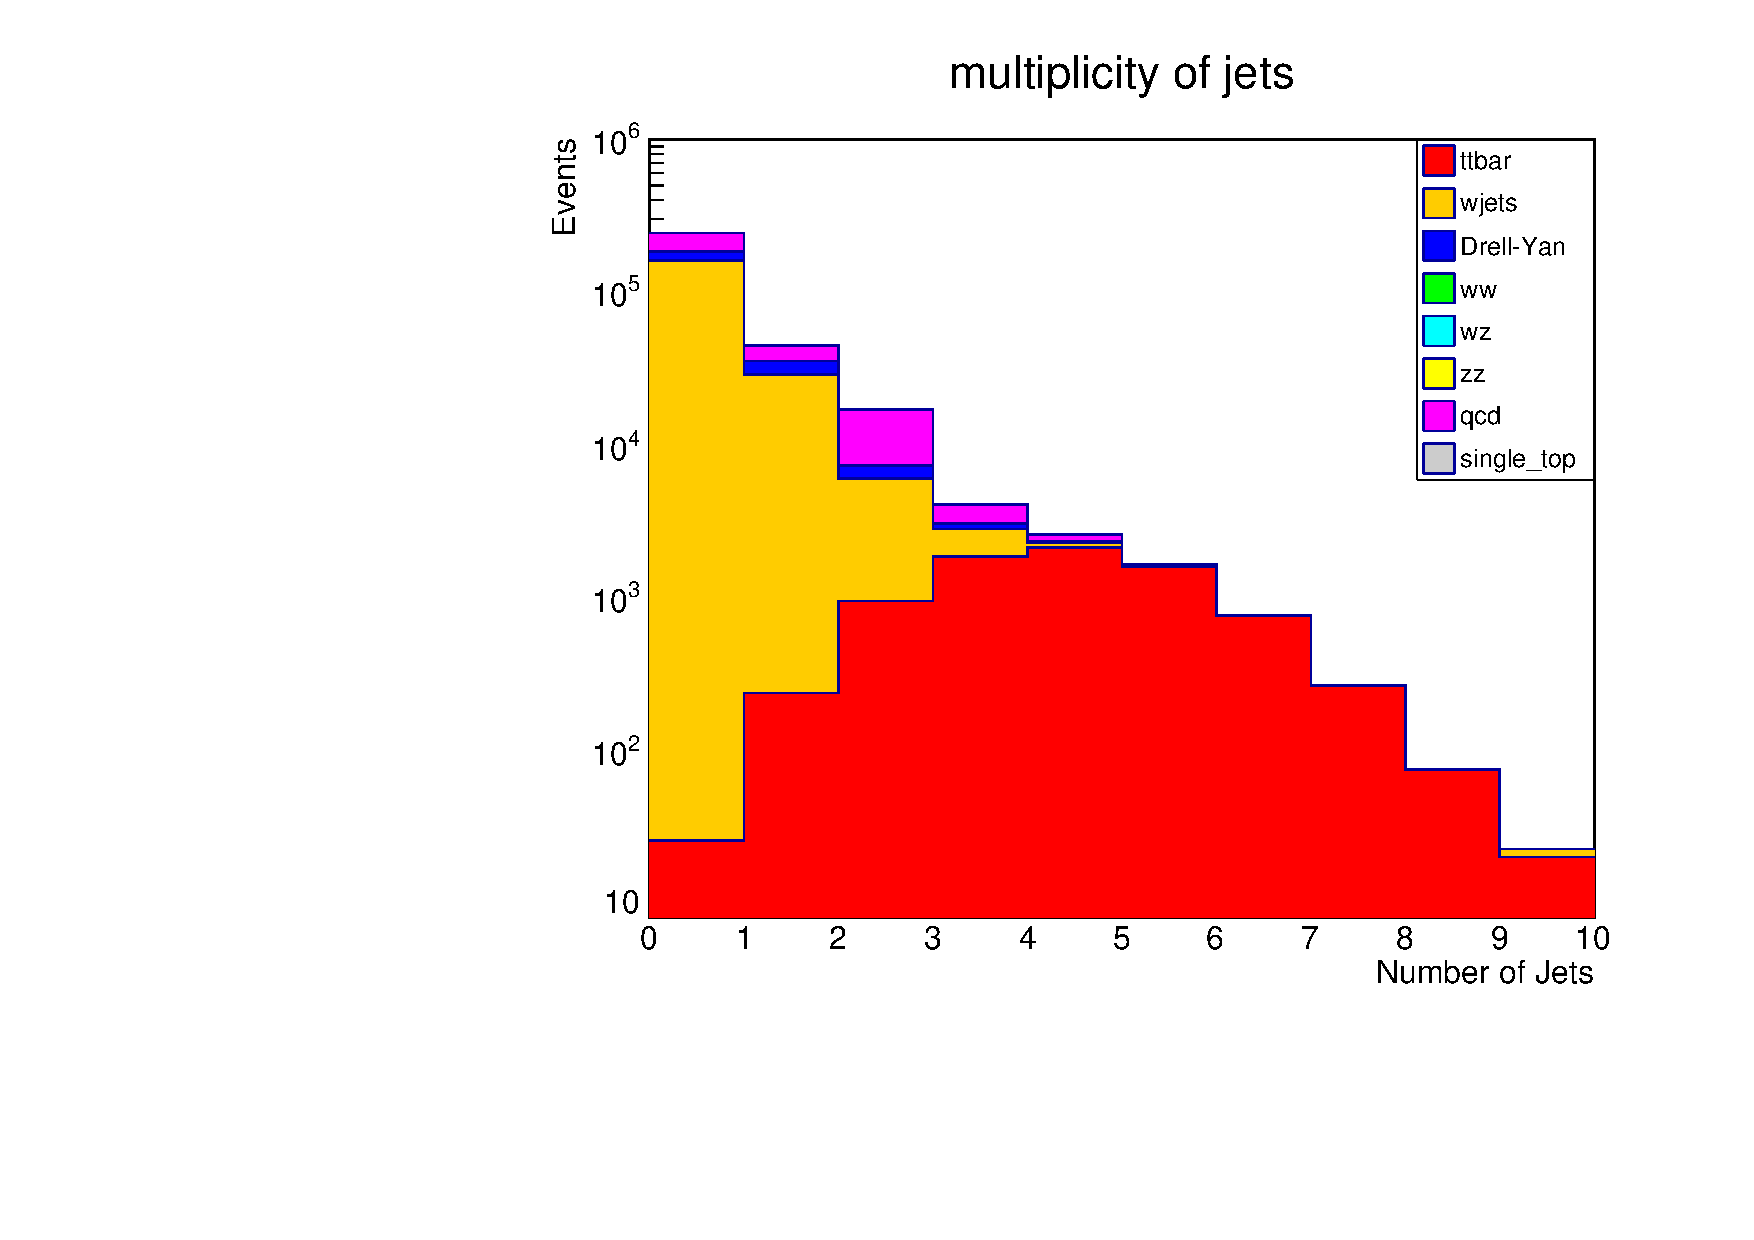
\includegraphics[width=7.5cm]{STACK_multi.pdf}
& 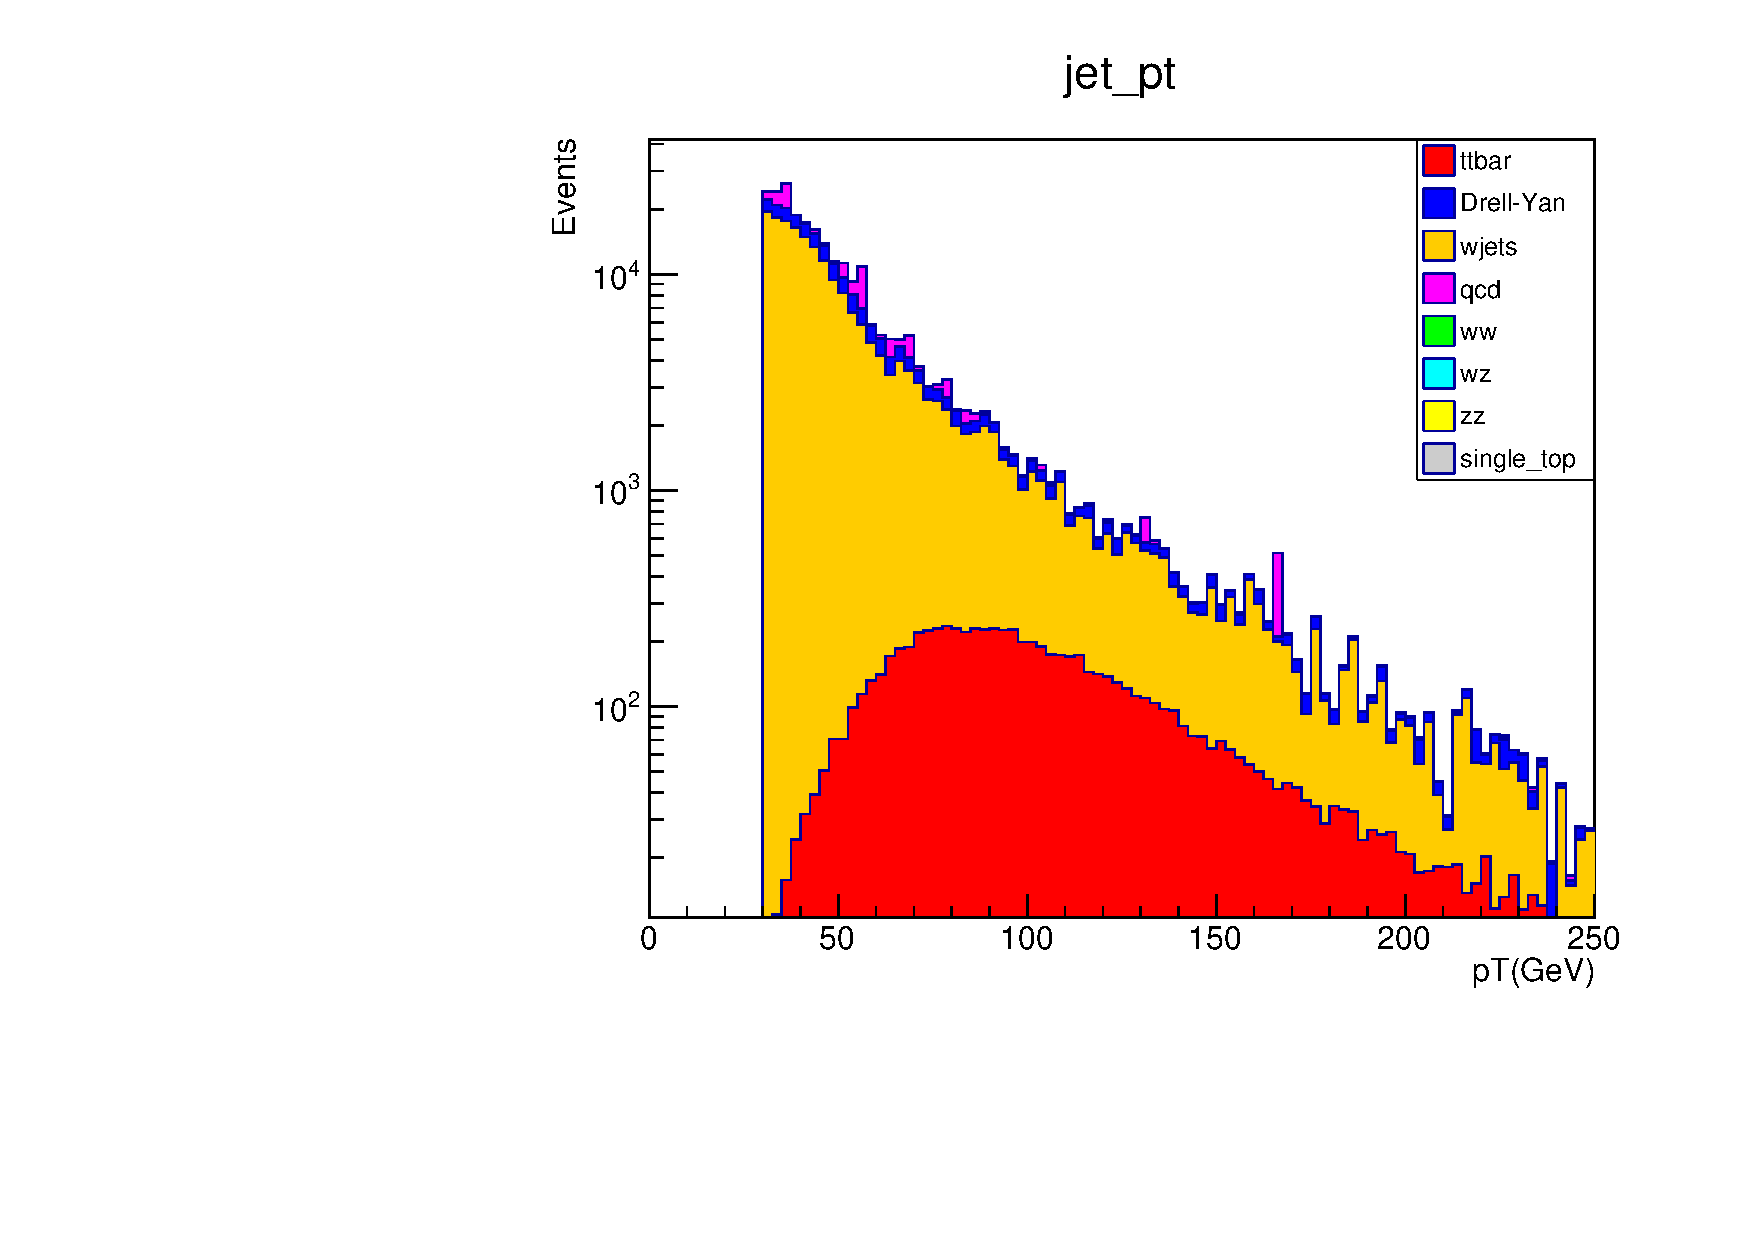
\includegraphics[width=7.5cm]{STACK_jet1_pt.pdf} \\
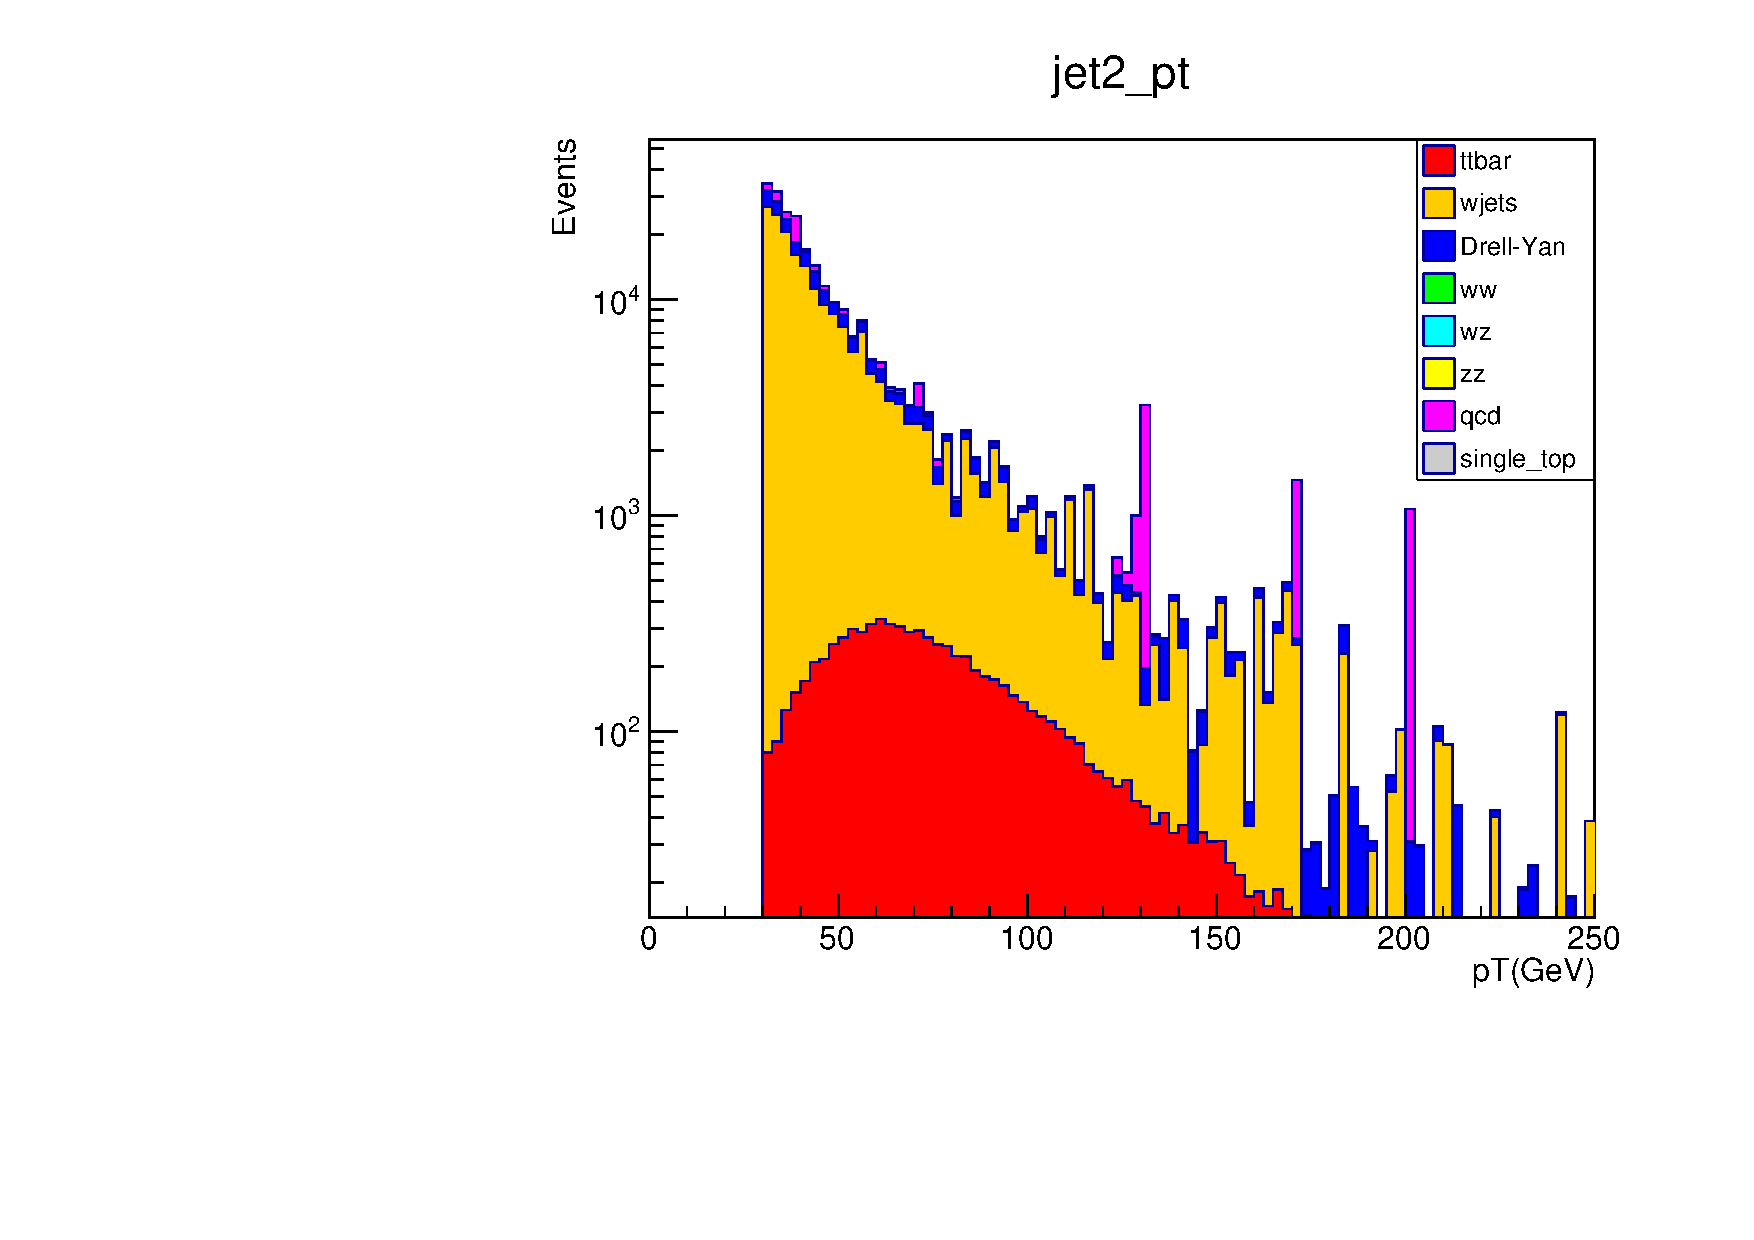
\includegraphics[width=7.5cm]{STACK_jet2_pt.pdf}
& 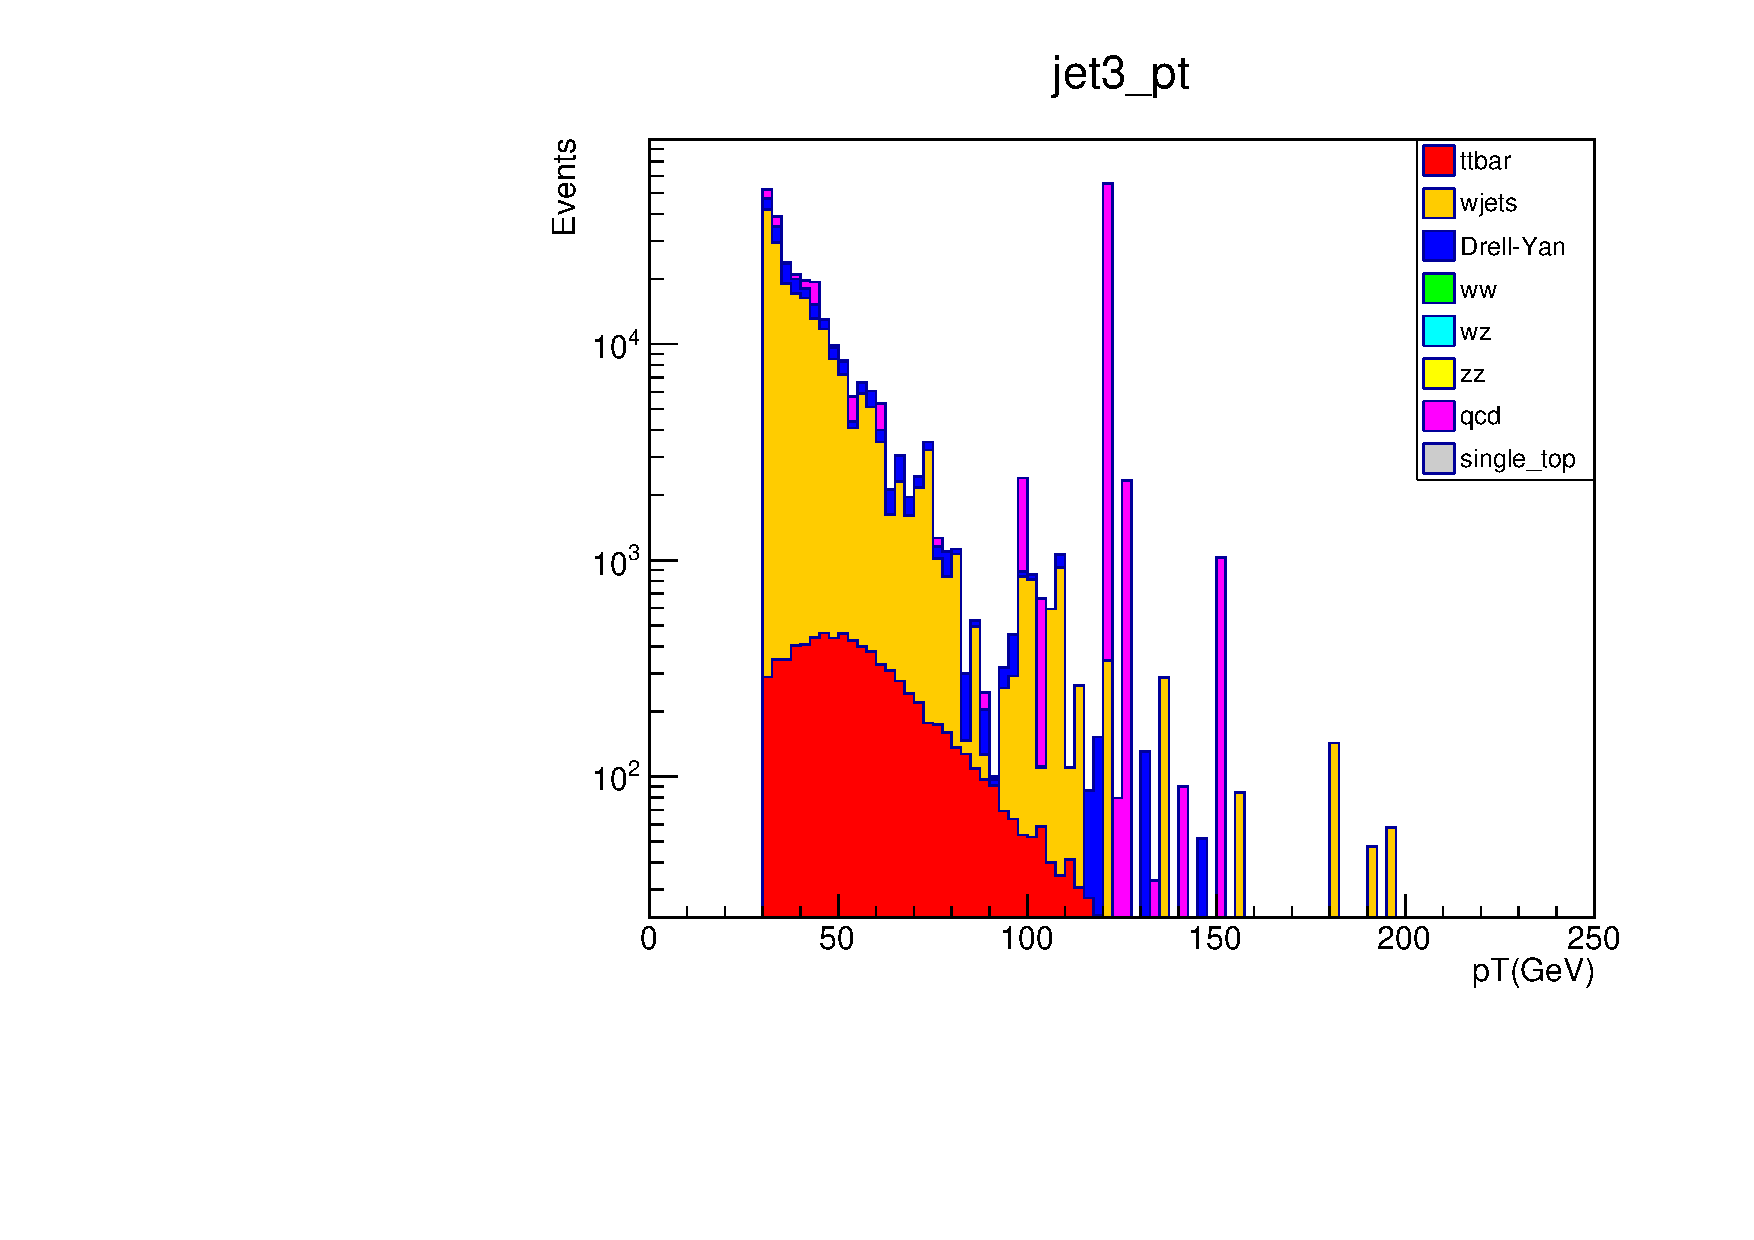
\includegraphics[width=7.5cm]{STACK_jet3_pt.pdf} \\
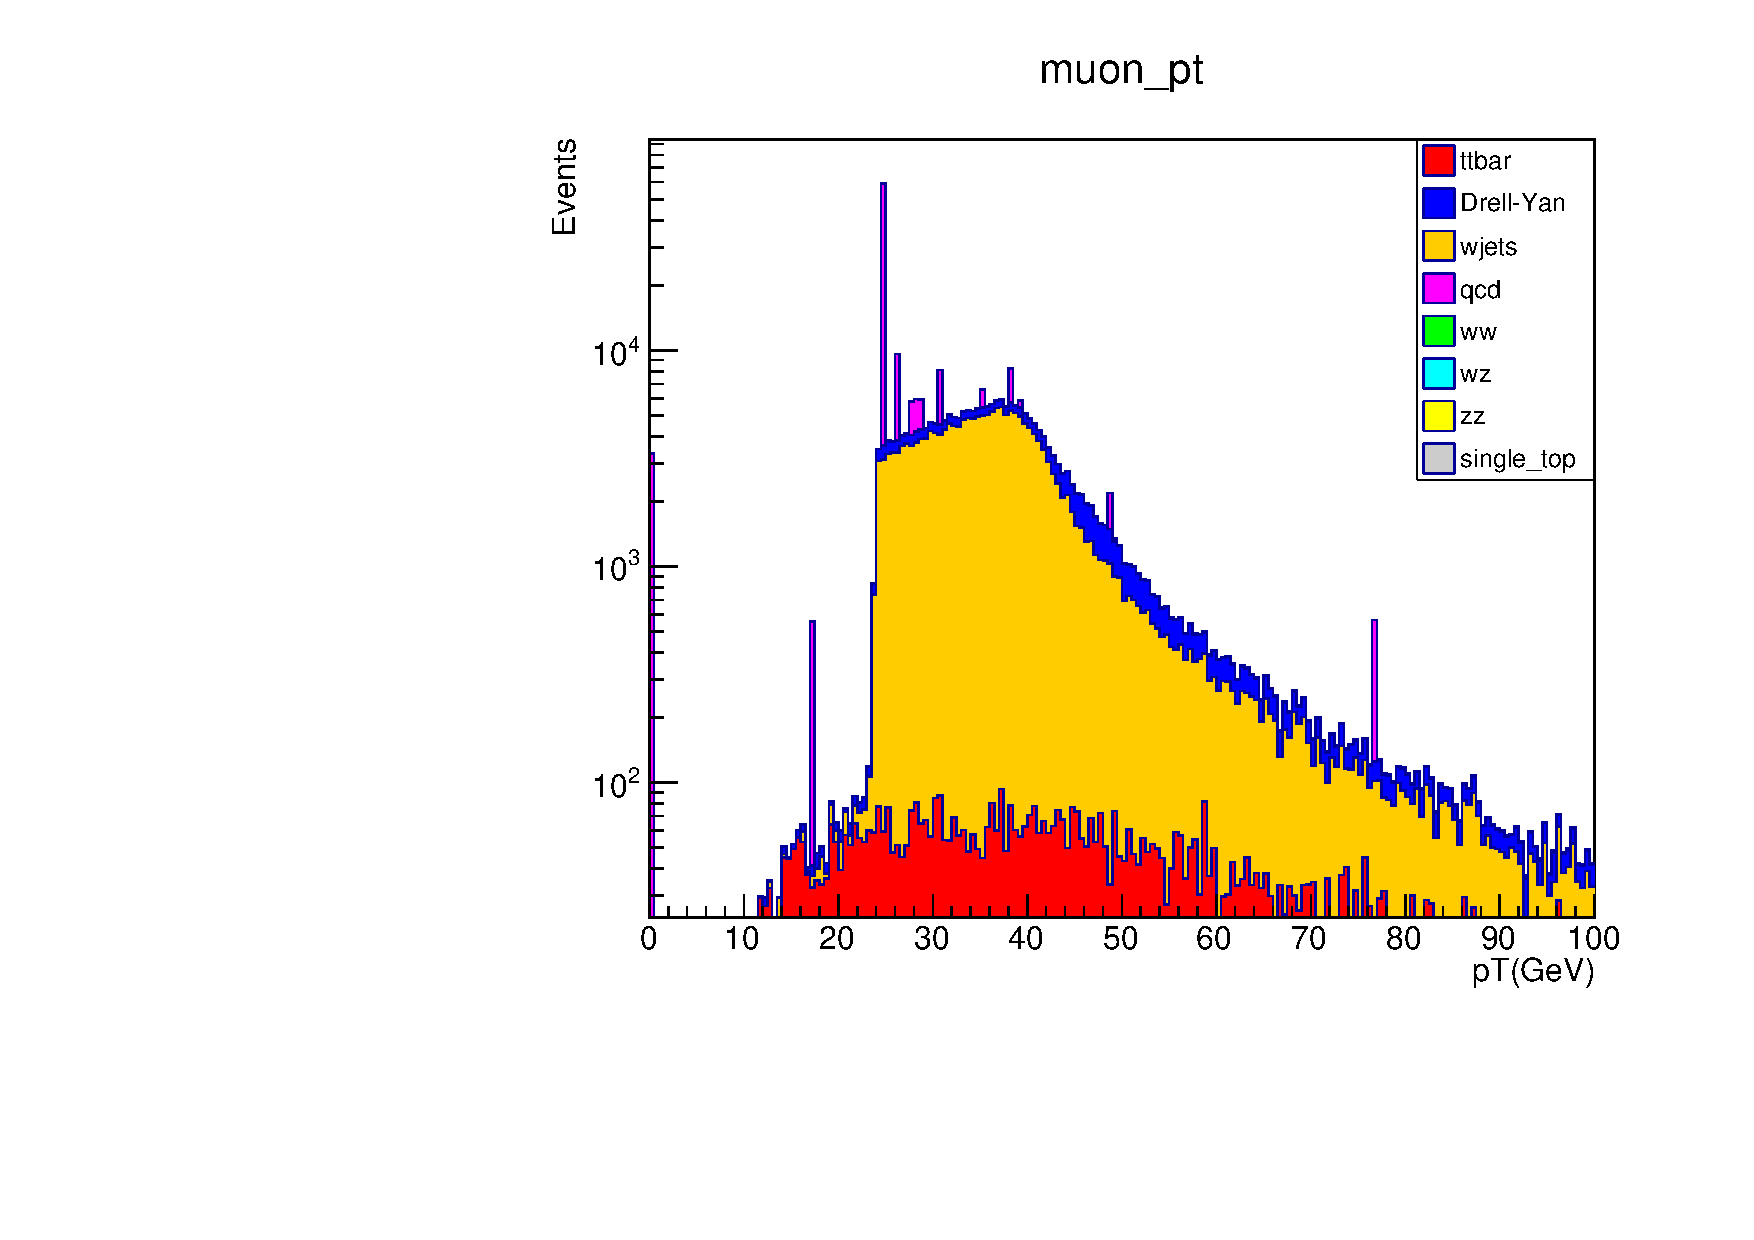
\includegraphics[width=7.5cm]{STACK_muon_pt.pdf}
& 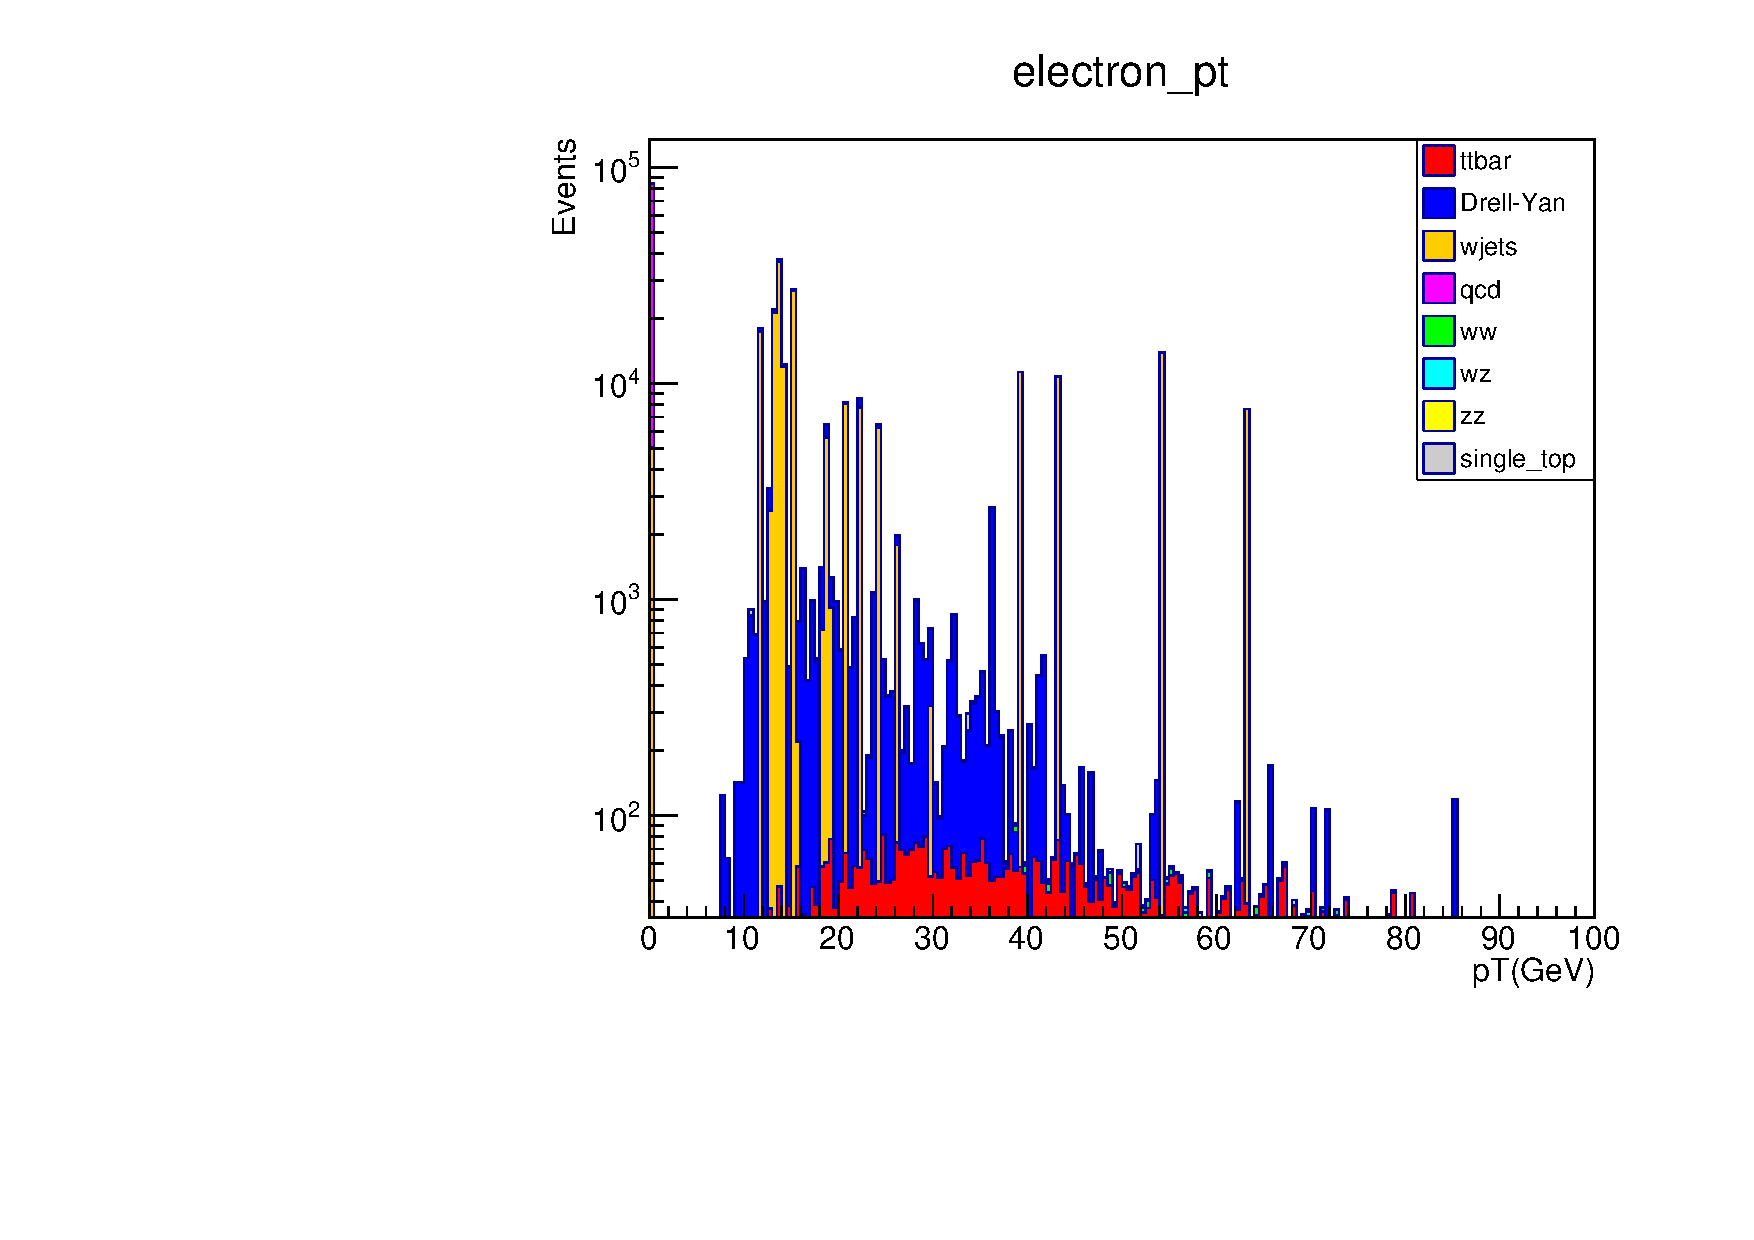
\includegraphics[width=7.5cm]{STACK_electron_pt.pdf}
\end{array}
\end{displaymath}
\newpage
\begin{displaymath}
\begin{array}{cc}
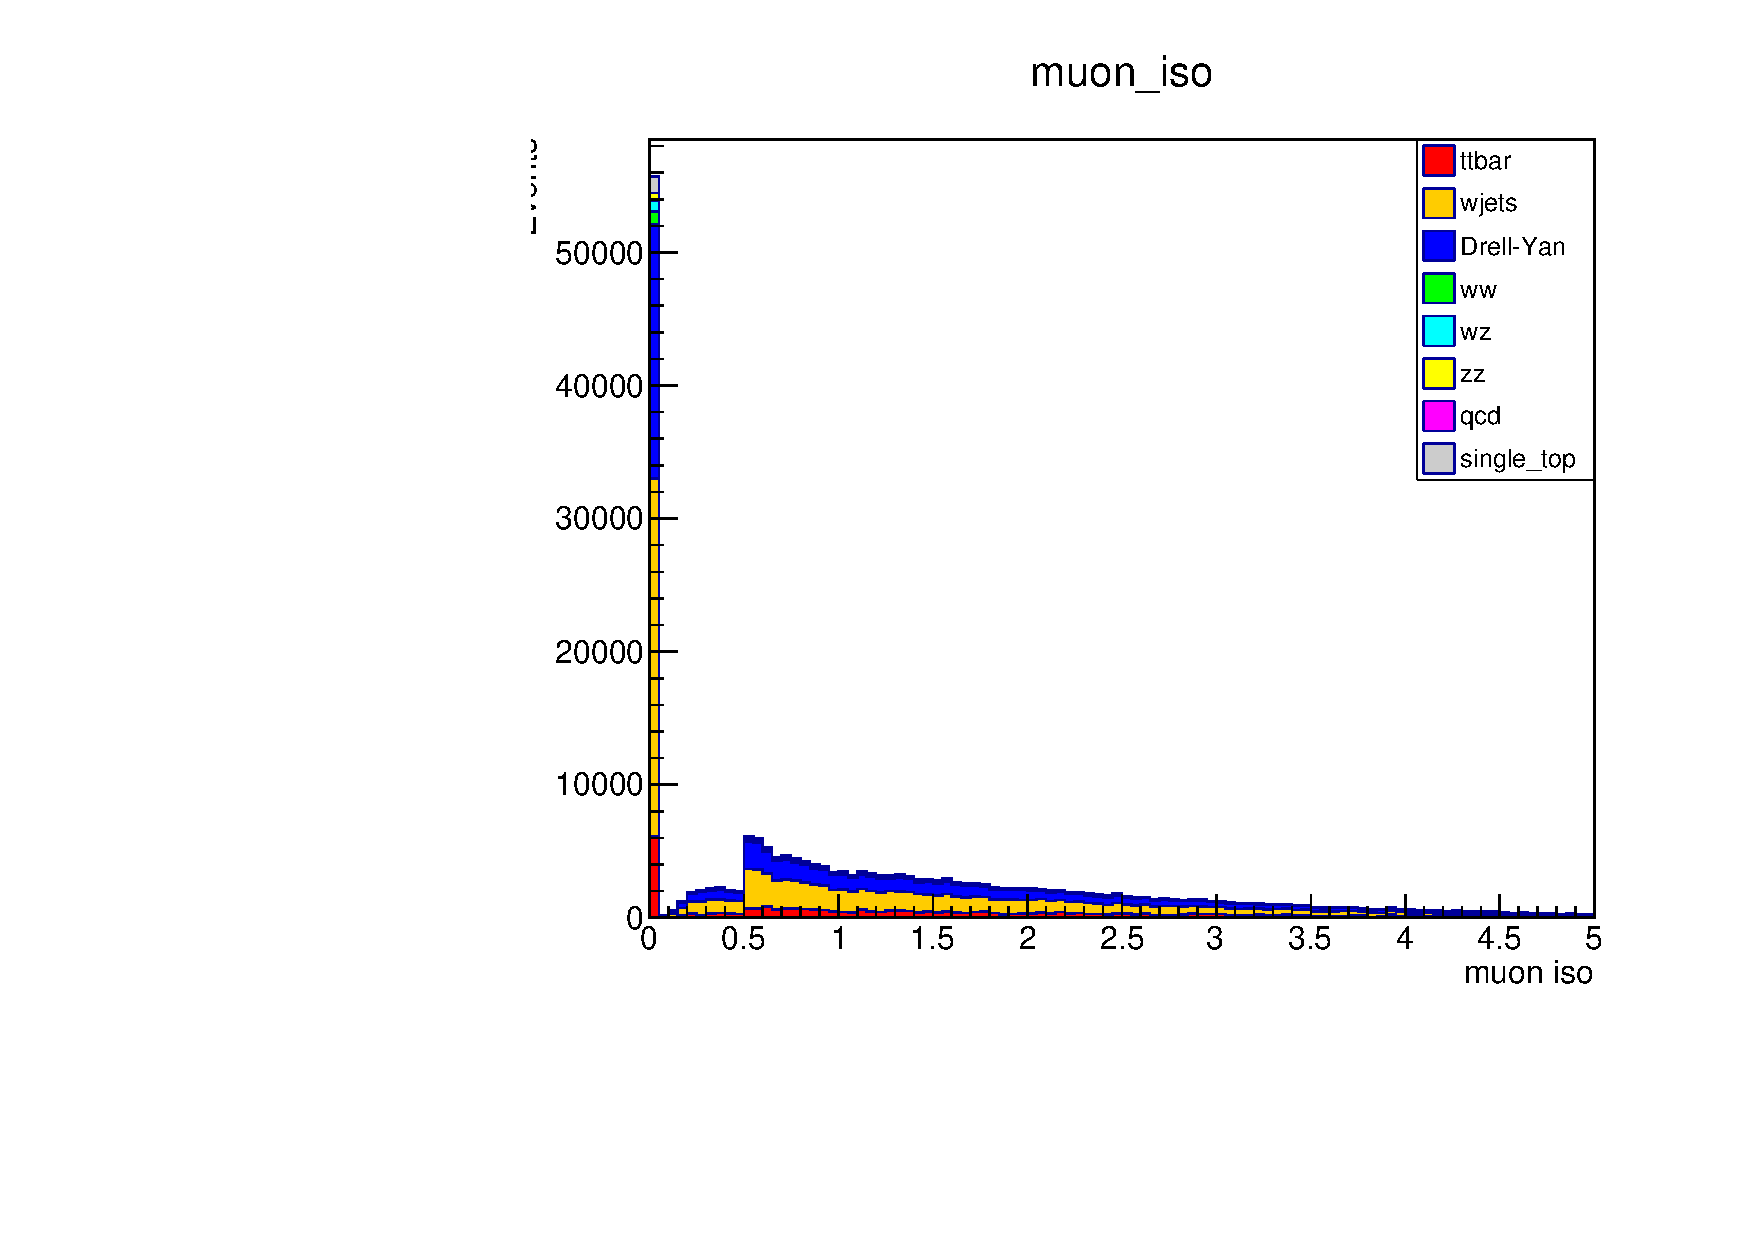
\includegraphics[width=7.5cm]{STACK_muon_iso.pdf}
& 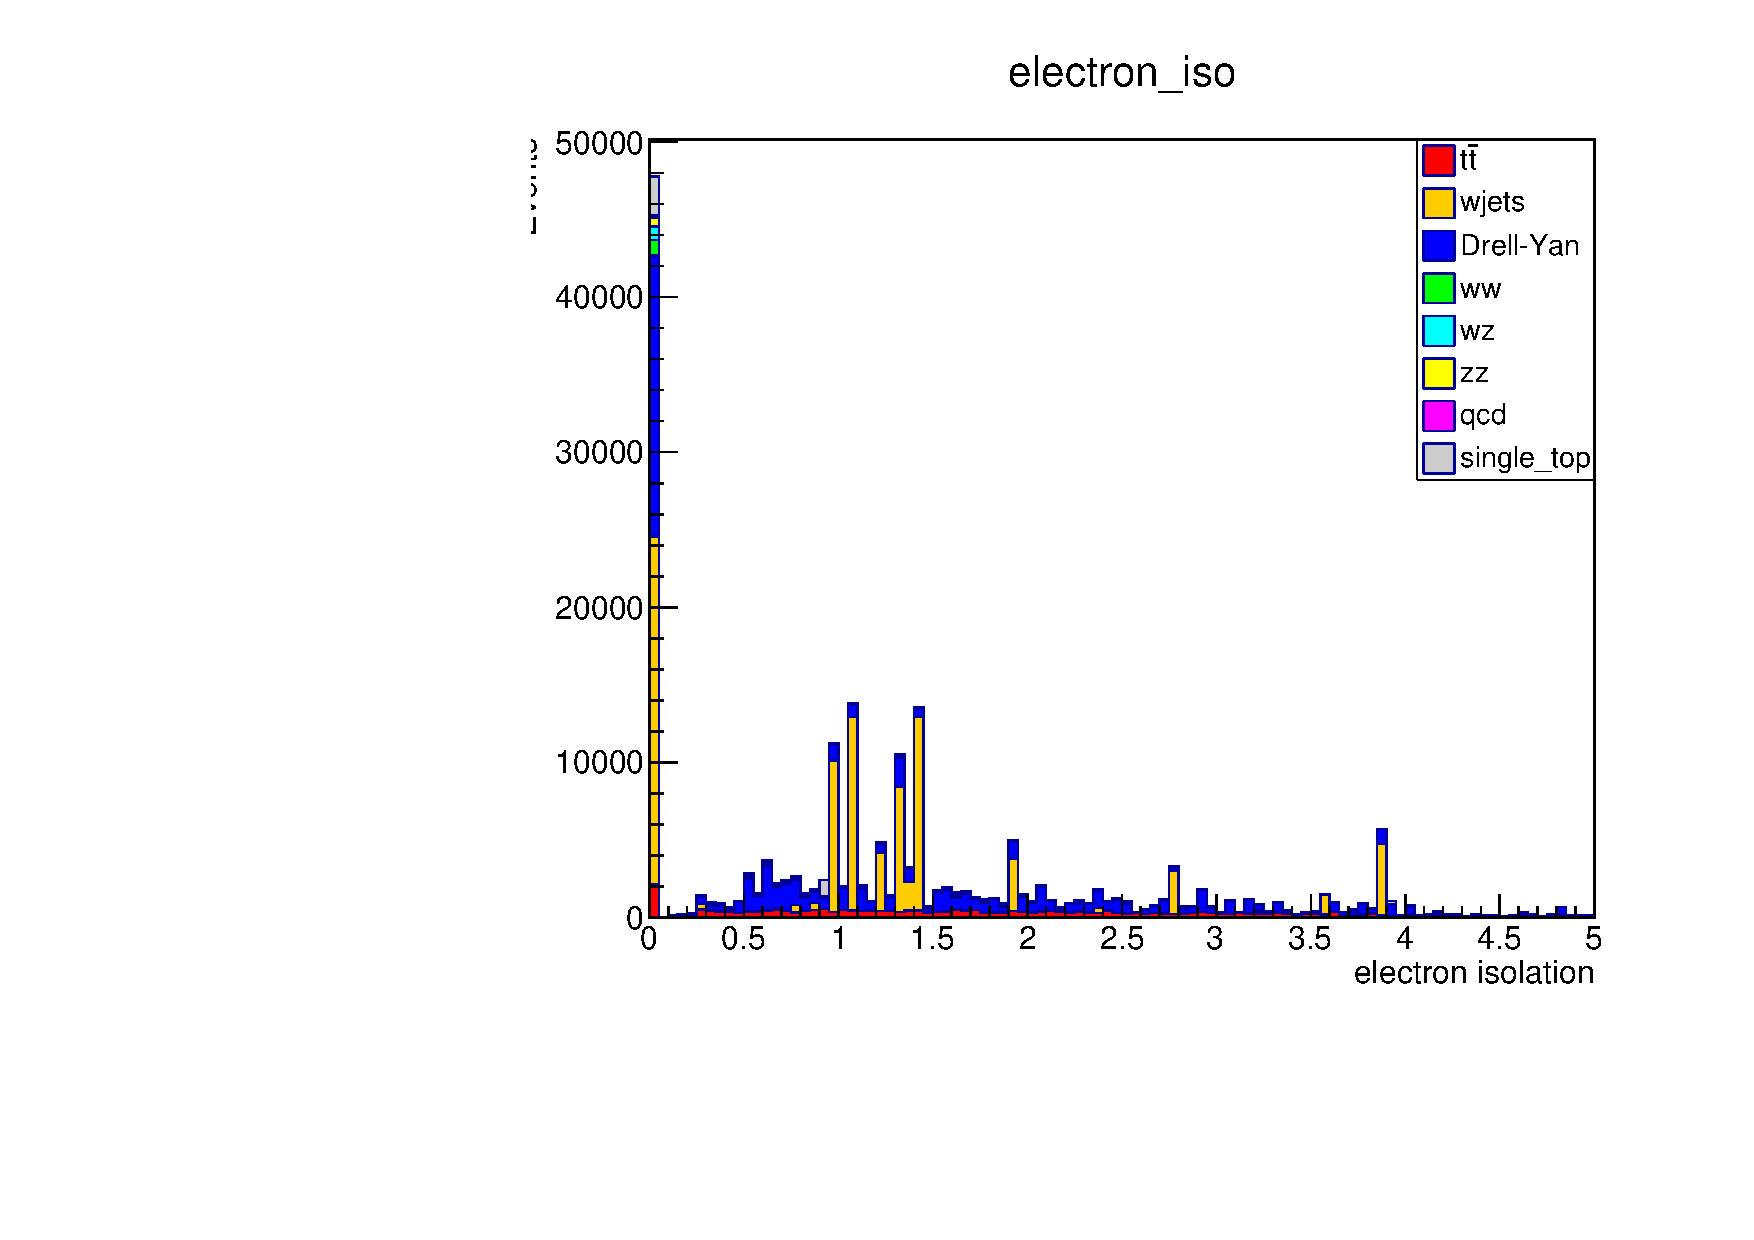
\includegraphics[width=7.5cm]{STACK_electron_iso.pdf} \\
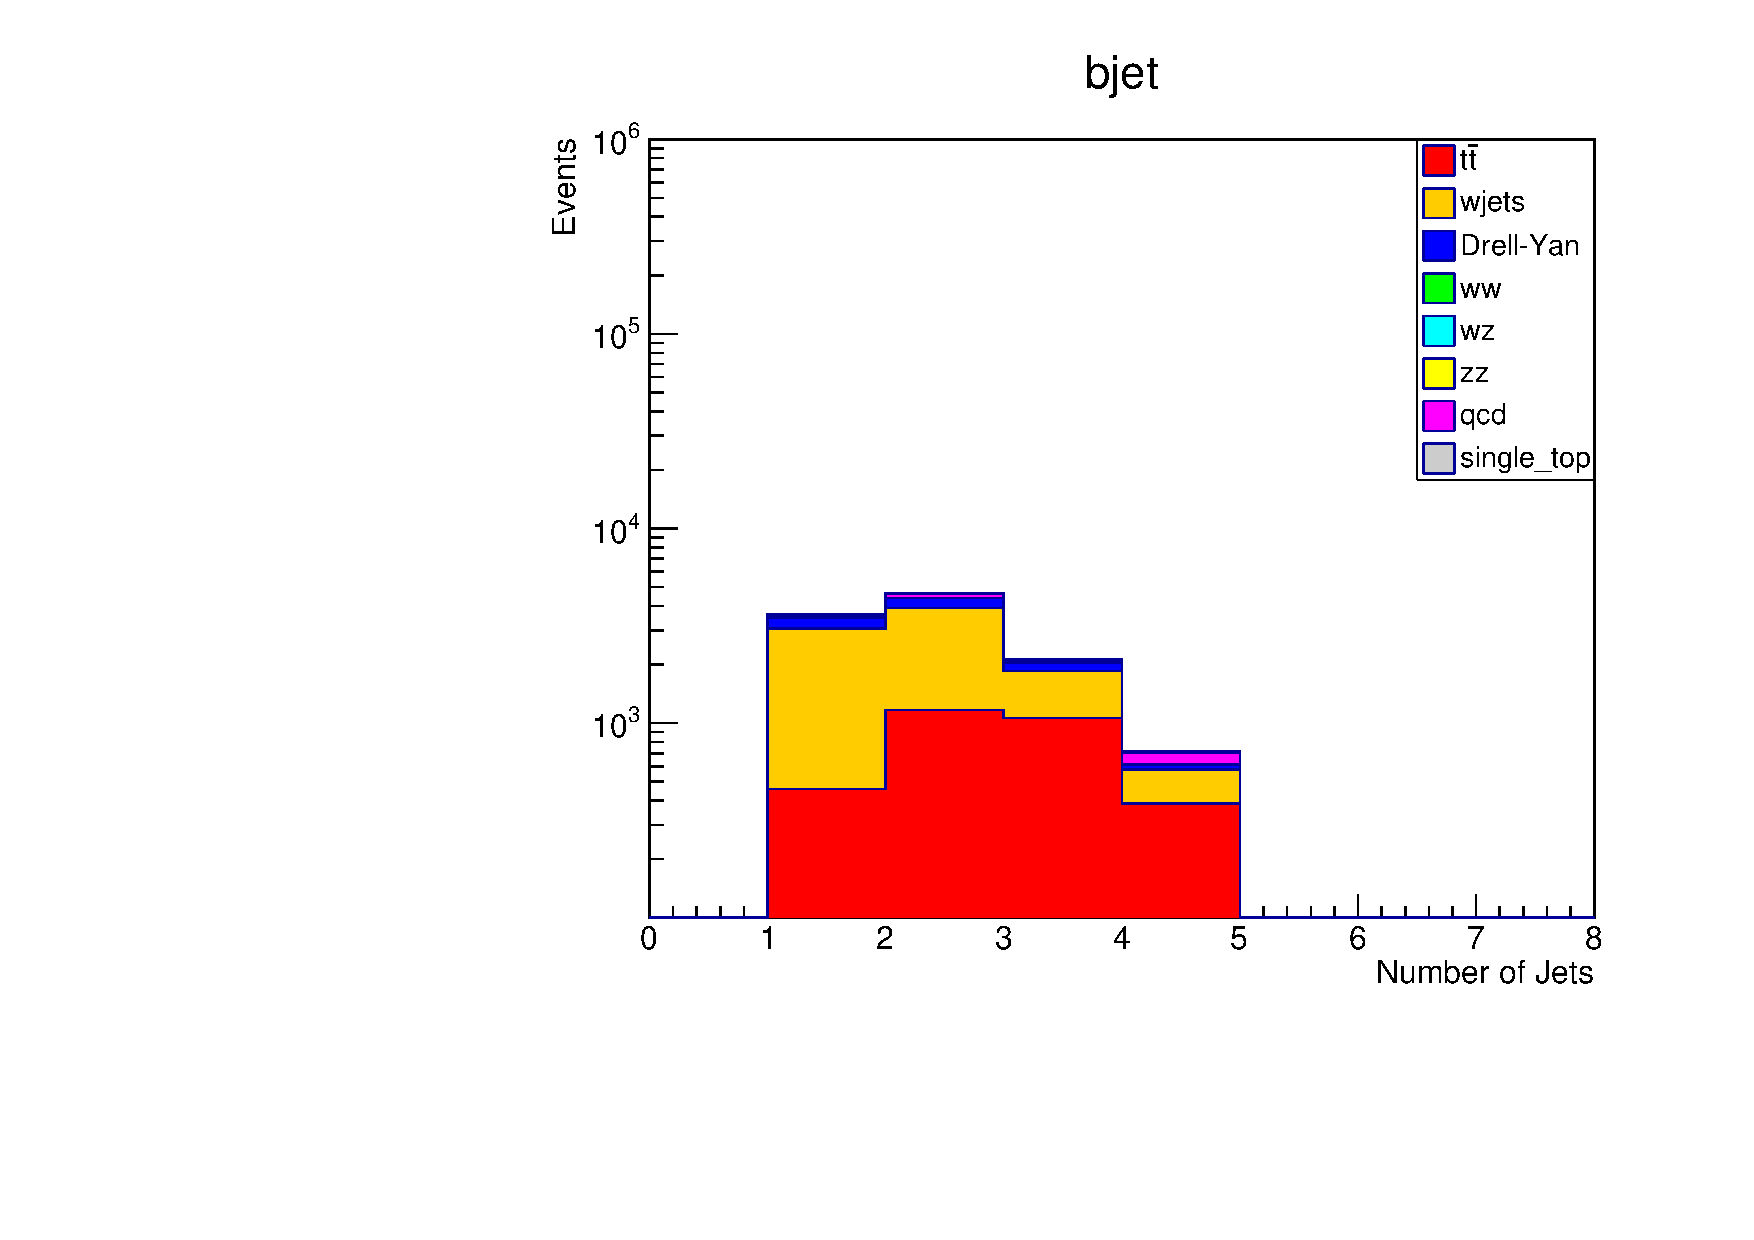
\includegraphics[width=7.5cm]{STACK_bjet.pdf}
& 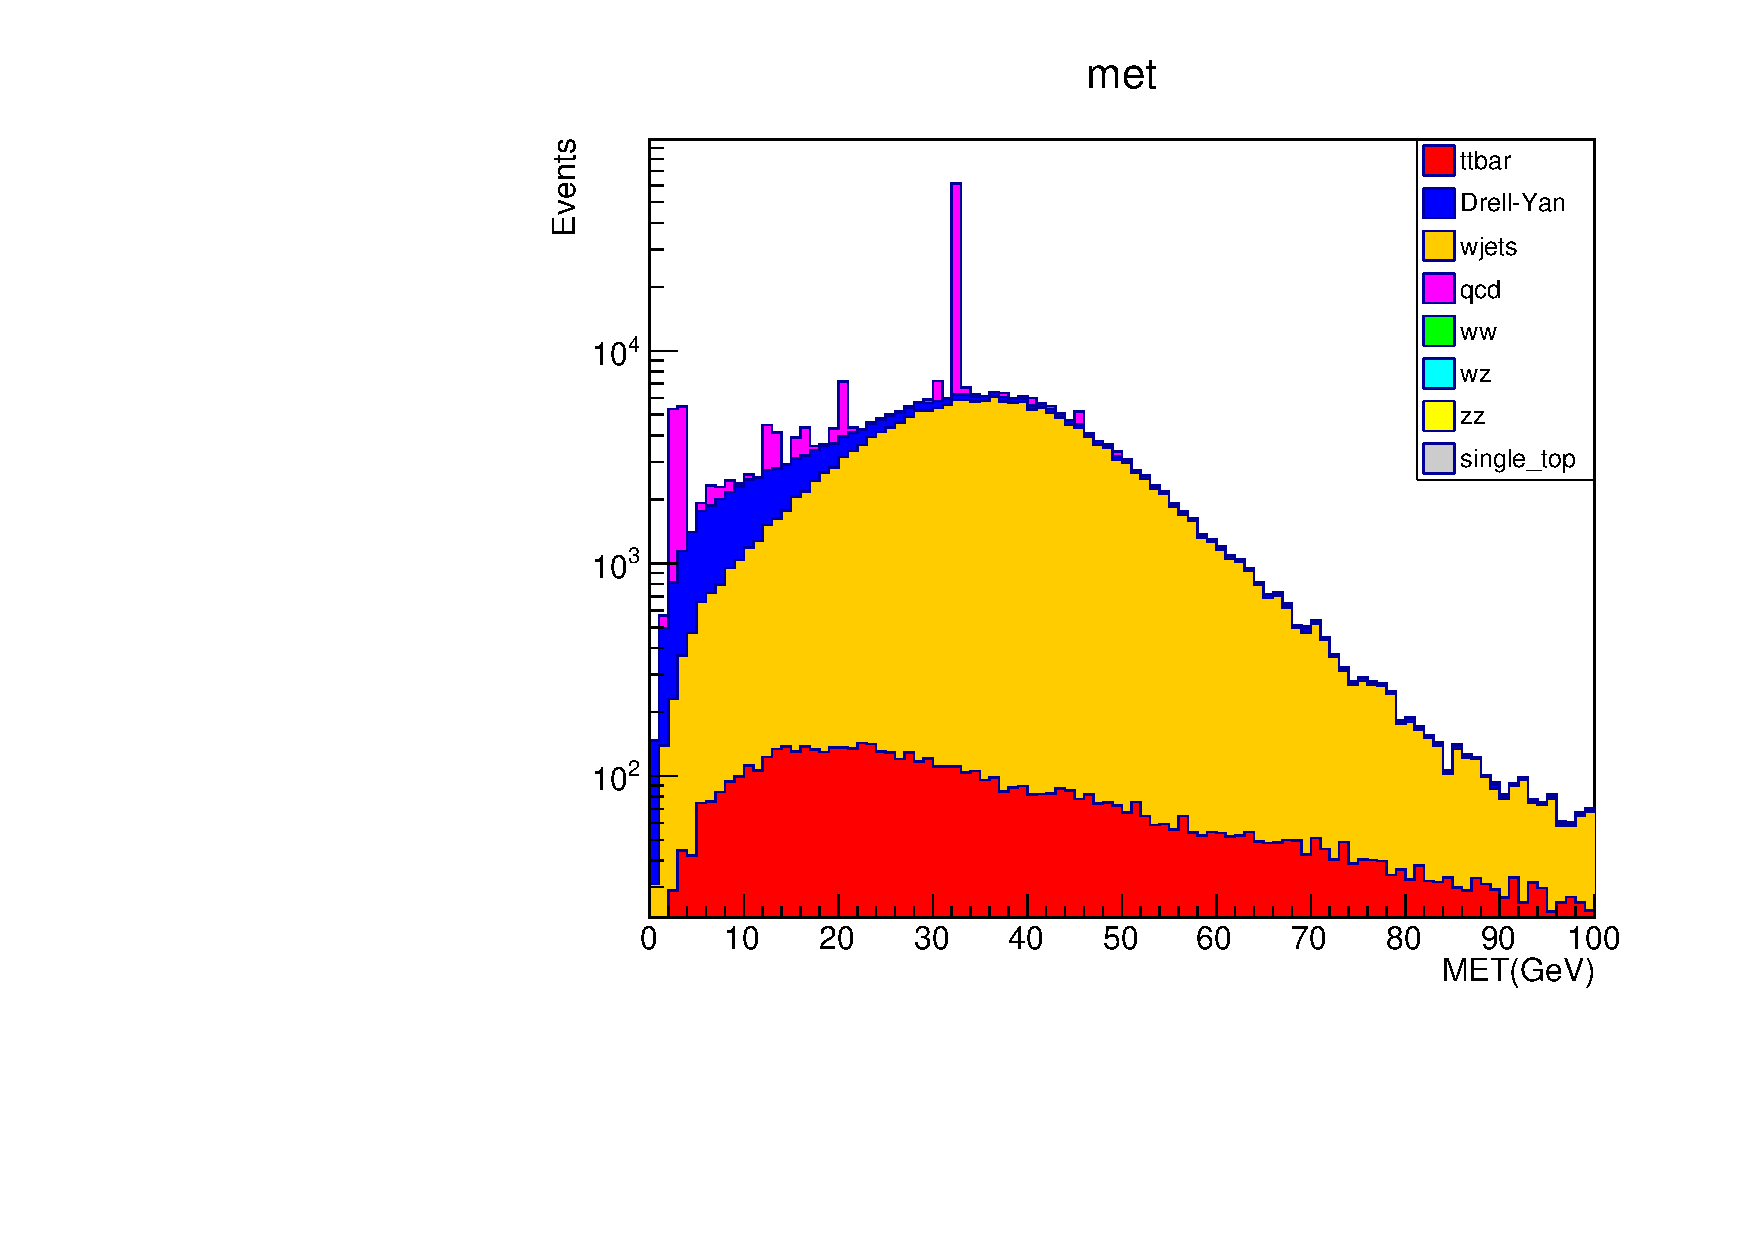
\includegraphics[width=7.5cm]{STACK_met.pdf} \\
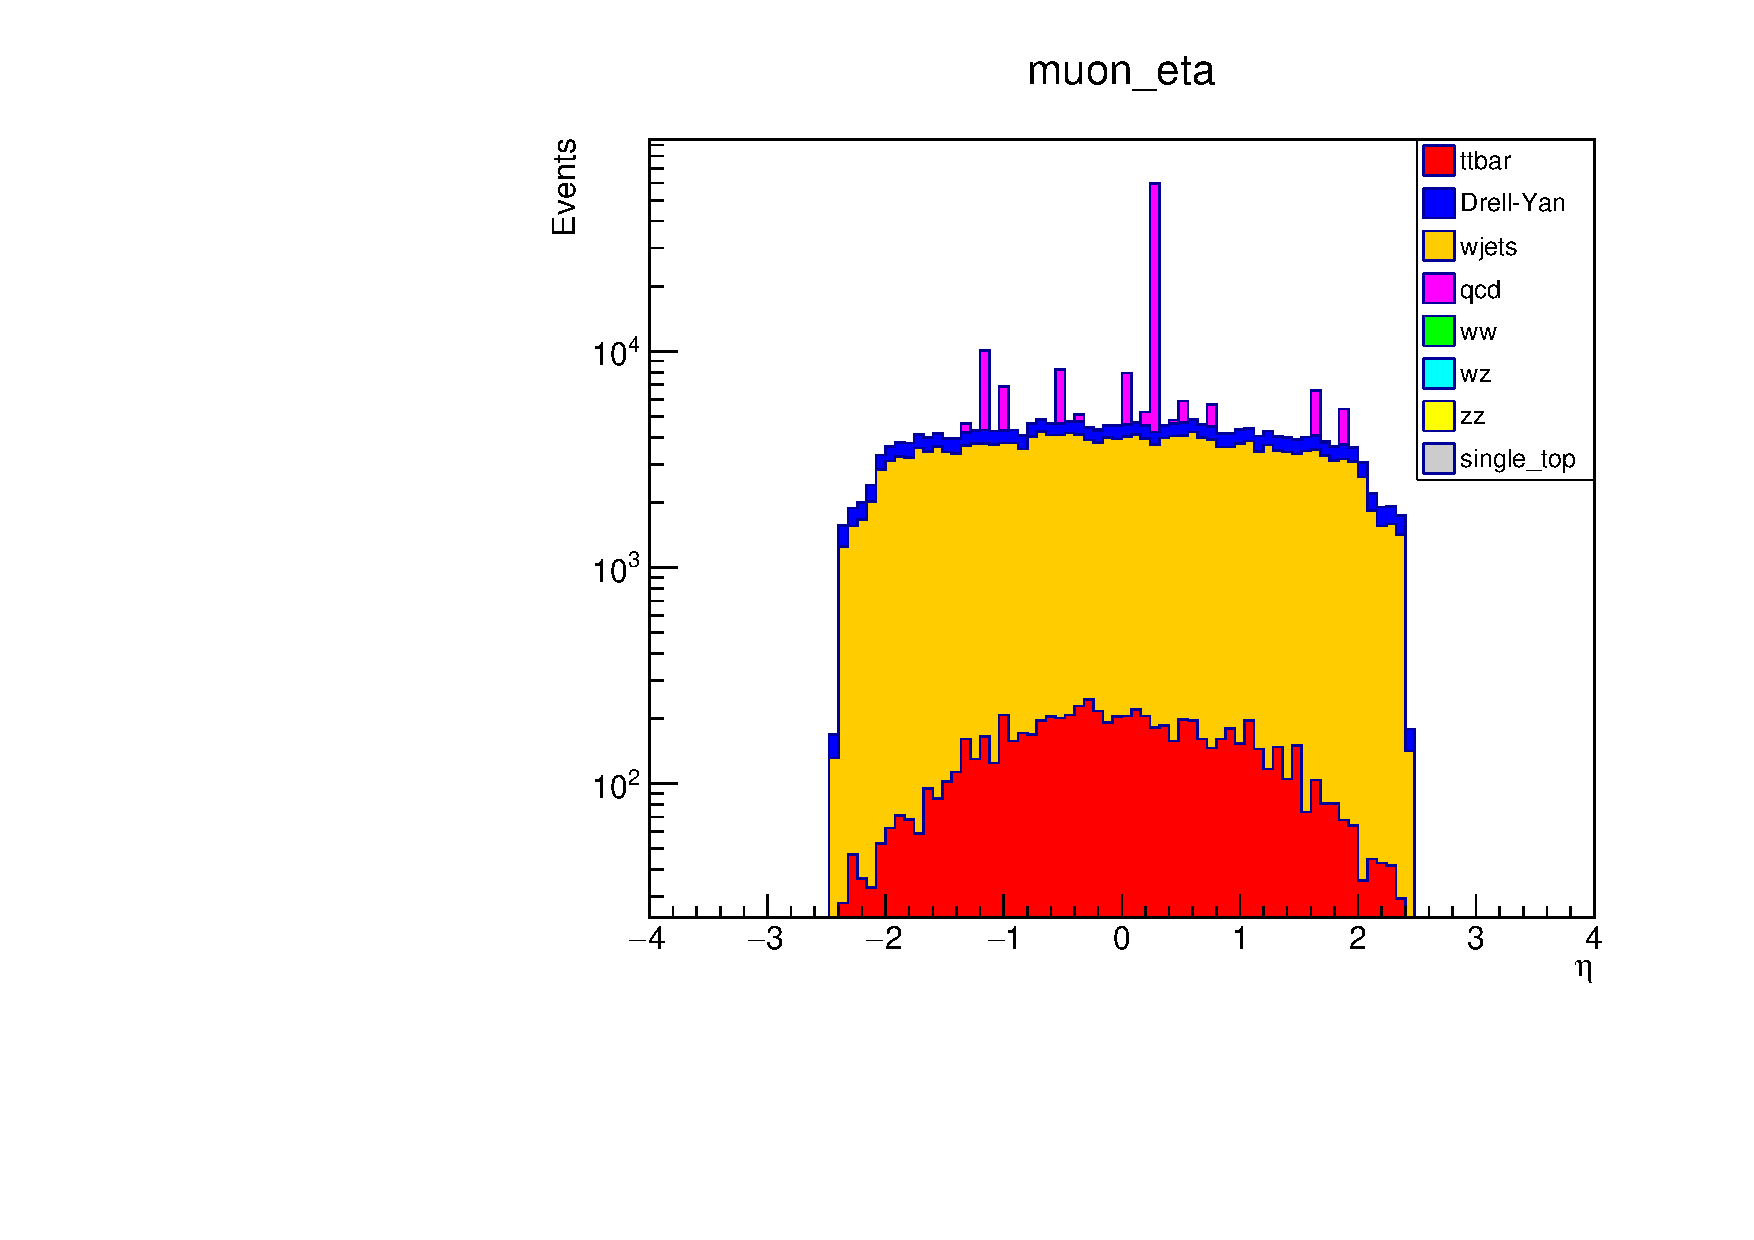
\includegraphics[width=7.5cm]{STACK_muon_eta.pdf}
& 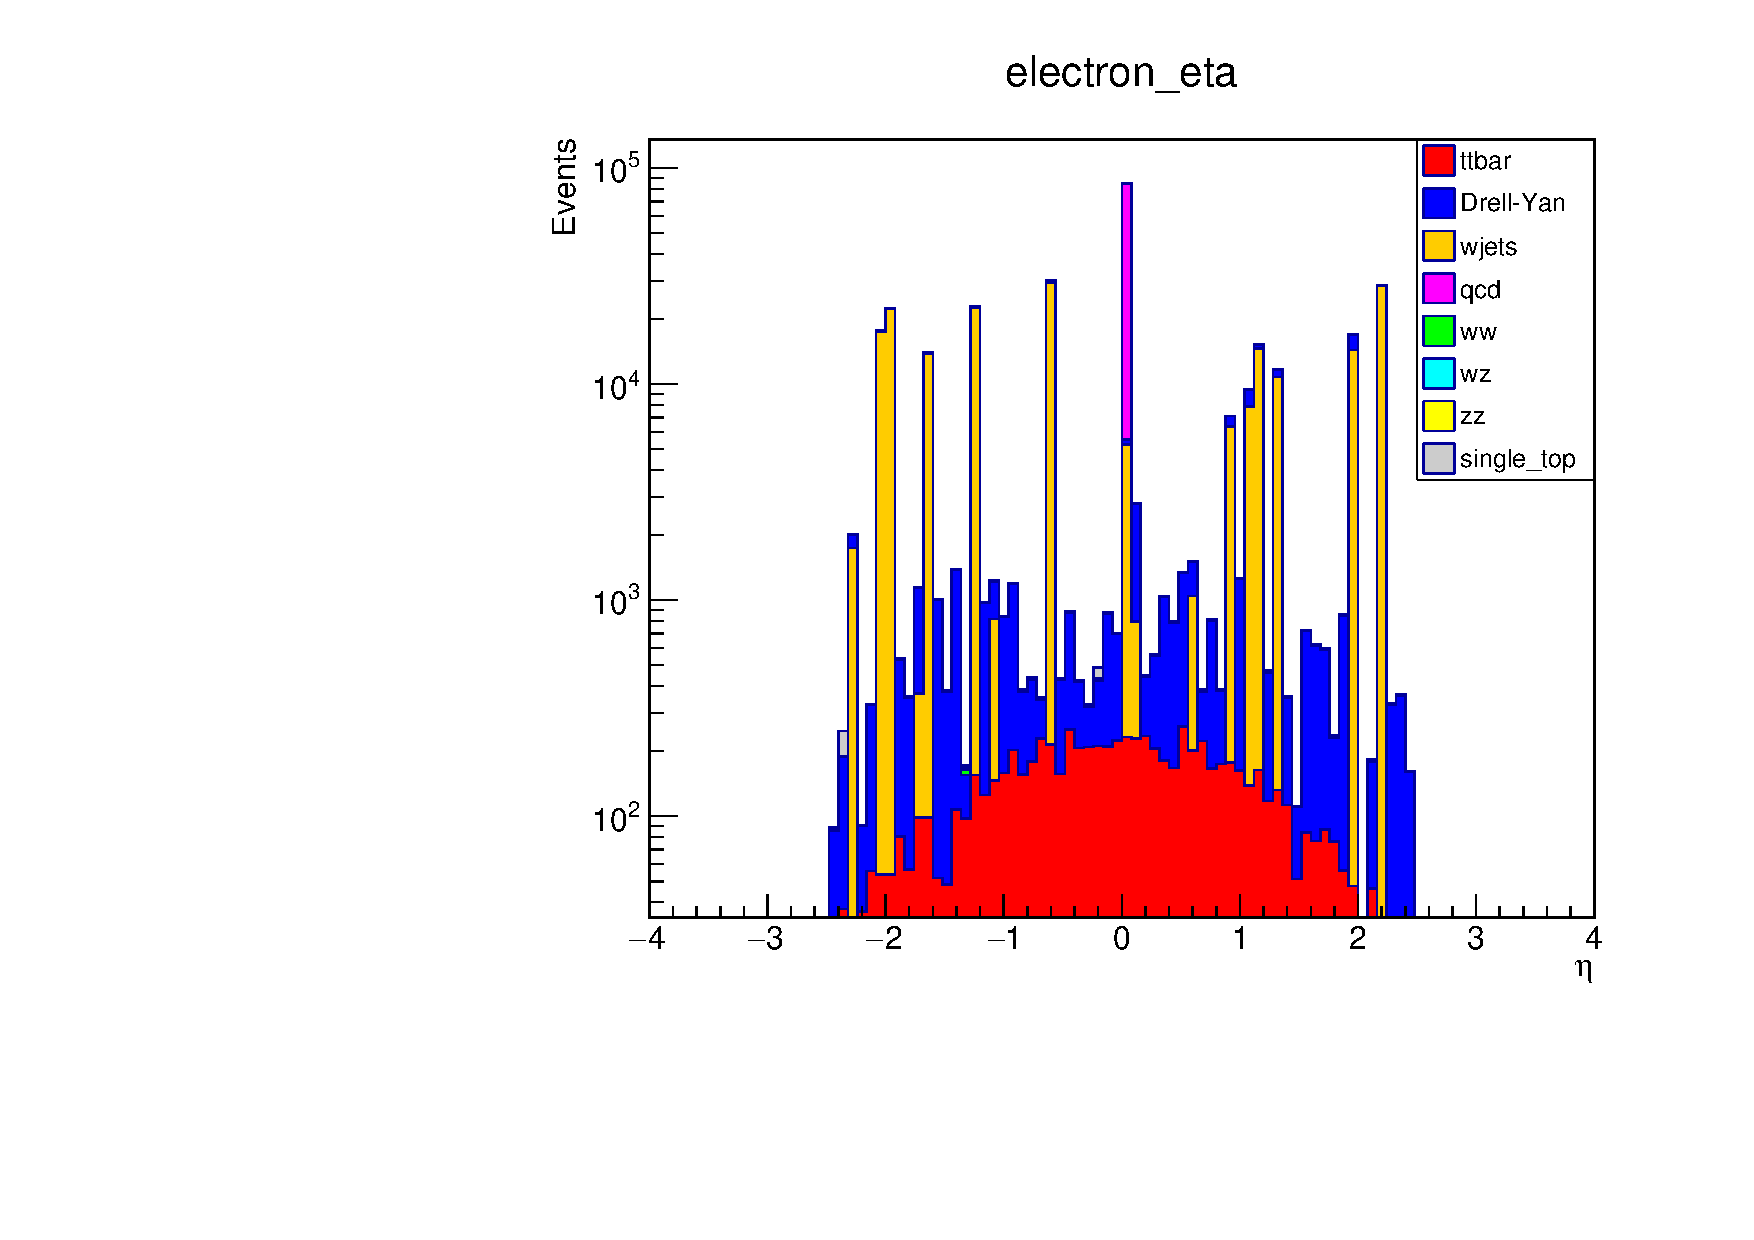
\includegraphics[width=7.5cm]{STACK_electron_eta.pdf} \\
\end{array}
\end{displaymath}

\newpage
\paragraph{2.2}
Try to find variables which are expecially sensitive to seperate signal from background (jet-multiplicity, transverse momenta of jets and leptons, lepton isolation, b-tagging, missing transverse energy, angular distributions). Fill all these distributions into histograms and compare between signal, background and data.

\begin{lstlisting}[emph={if,while,continue,new},emphstyle=\color{nut}]

\end{lstlisting}


\newpage
\paragraph{2.2}
Try to find variables which are expecially sensitive to seperate signal from background (jet-multiplicity, transverse momenta of jets and leptons, lepton isolation, b-tagging, missing transverse energy, angular distributions). Fill all these distributions into histograms and compare between signal, background and data.

\newpage
\paragraph{2.3}
Apply cuts on these variables to enrich the signal over background. Try to optimize the signal over background ratio and estimate the purity that can be achieved (based on simulation only).

\newpage
\paragraph{2.4}
Apply your selection cuts also on data. Compare the selection efficiency between data and simulation.

\end{document}
